\section{Future Work}
\subsection{Touch-down angle of attack control strategy}\label{TDcontrol}
Although in sections (\ref{walkingmodel}) and (\ref{simulation}) a constant angle of attack policy was introduced, it is possible to have a dynamical control of this parameter so that after 2 strides the system is found in a stable setup.  As discussed in \cite{Carver2009}, a single step is insufficient for the system to have a stabilizing an equilibrium gait, therefore, by implementing a two step control policy, we have ensured stable walking in the minimum number of steps. Such type of control is also called deadbeat control policy. This is done in \cite{Vejdani2015}, using a feedback control technique that sends the next step of the system into a stable walking gait. Supposing we have an equilibrium state $(\psi^*,\theta^*)$ which we want to achieve, we can find the two stride region of attraction $[y,\beta]$ if we find a state $\psi_n$ which satisfies
\begin{equation}
  A(\psi_n,\theta_n)=\psi_{n+1},
  \label{eq.psi1}
  \end{equation}
\noindent where A is the system which iterates the next poincare section with Eqs. (\ref{eq.singlesuppx})-(\ref{eq.doublesuppy}),
\begin{equation}
  A(\psi_{n+1},\theta_{n+1})=\psi^*.
  \label{eq.psi+1}
\end{equation}
\noindent If relations \ref{eq.psi1} and \ref{eq.psi+1} are satisfied, the system will converge to $\psi^*$ in the fastest number of steps (deadbeat control policy). This way, the angle that is chosen for the next iteration is, given through the invertion of the combination found in Eqs. (\ref{eq.psi1}) and (\ref{eq.psi+1}), 

\begin{equation}
  \theta_n=\left.A^{-1}\right|_{\psi_n}(\psi_{n+1})
\end{equation}
where the existence of a valid intermediate state $\psi_{n+1}$ is assured by constructing a two-step domain. Notice that eventhough, it is necessary to obtain a value for $\theta_{n+1}$, to compute $A(\psi_{n+1},\theta_{n+1})$, in practice this value is not used to compute the next iteration of angle of attack but to filter the states in which $A(\psi_{n+1},\theta_{n+1})=\psi*$.



\subsection{2 spring model for running and walking}\label{2springssection}
To contemplate a more realistic model, throught this thesis i plan on developing a more realistic model for running robust for noise compared to section (\ref{hoppingmodel}). It consists on two springs with spring stiffness $k1$ and $k2$, and 3 masses, m1, m2, m3, the angle velocity makes with the ground is defined by $\gamma_0$ and $\vec{v_0}$ is the initial velocity vector. Figs. (\ref{2spring1})-(\ref{2spring3}) displays the 3 control phases and important variables to the model. 

\begin{figure}[H]
   \centering
   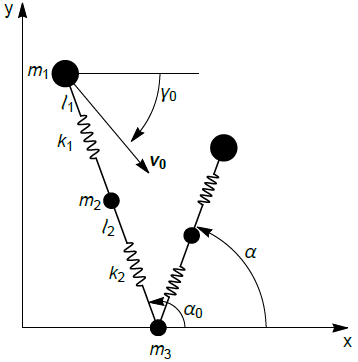
\includegraphics[width=0.4 \textwidth]{initialphase}
   \caption{Phase-I of the 2 spring model, ground phase to aerial phase. With no bending, the leg rotates around it's pivot located on the ground similar to section (\ref{hoppingmodel}). Upon reaching the angle $\alpha$ the model starts the phase II, aerial phase.}
   \label{2spring1}
  \end{figure}

\begin{figure}[H]
  \centering
  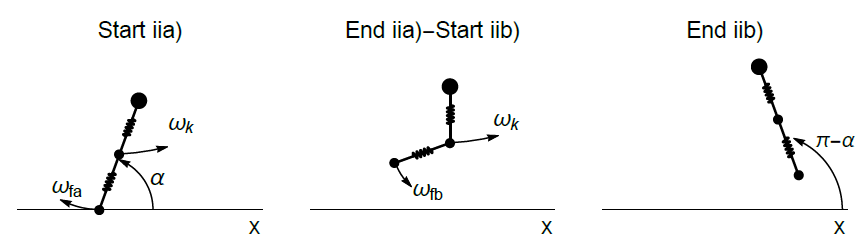
\includegraphics[width=0.9 \textwidth]{secondphase}
  \caption{Phase-II of the 2 spring model, aerial phase. Part a) of this phase involves rotating the rotor in the joint, so that a torque is applied to the second part of the leg making it move in the clockwise orientation. At the same time, a torque is also applied to the first part of so making it rotate in a counter-clockwise orientation. With this, when the first part of the leg reaches it's vertical orientation the second part of this phase starts. Part b) is about moving the leg so that it becomes aligned with with an angle of $\pi-\alpha$. }
  \label{2spring2}
\end{figure}

\begin{figure}[H]
  \centering
  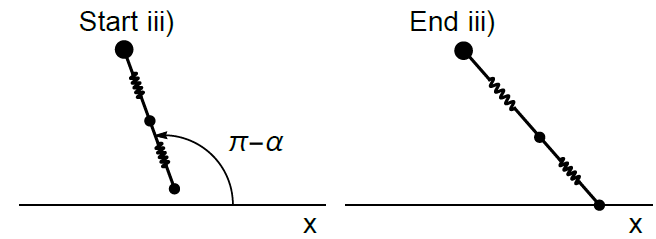
\includegraphics[width=0.6 \textwidth]{thirdphase}
  \caption{Phase III of the 2 spring model, aerial phase to ground phase. With the leg distended, free fall starts so that the leg contacts the floor so that phase I starts again.}
     \label{2spring3}
  \end{figure}

Using a similar kind of mechanism to section (\ref{TDcontrol}), i pretend to make a model  which is capable of finding the region of attraction so that it is adaptative to initial conditions and obstacles such as stairs. This way, one of the objectives will be to analyze the stability of the parameters described, this is, the strong and weak points of this model.

Besides a running model, i will also plan to implement a walking model with joints but with double support and single support phases similar to section (\ref{walkingmodel}). 
